\documentclass[aspectratio=169]{beamer}
\usetheme{Hannover}
\usecolortheme{magpie}
\beamertemplatenavigationsymbolsempty
\usepackage{graphicx}
\graphicspath{{images}}
\usepackage{tikz}
\usepackage{pgfplots}
\title{{\it I Wanna Be Like You}}
\subtitle{Robust \& Rapid Emulation for Efficient Trial Design}
\author{Jack Fraser-Govil}
\date{23/03/26}
% \logo{
\includegraphics[scale=0.3]{crest3}}
\makeatletter \addtobeamertemplate {sidebar left} {}{ 
\includegraphics [width=\beamer@sidebarwidth]{crest3}} \makeatother 

\renewcommand{\vec}[1]{\mathbf{\boldsymbol{#1}}}
\def\pitem{\pause\item}

\begin{document}
    \maketitle

    \section{Why Emulate?}
        \begin{frame}{Why do we want to Emulate?}

            \begin{itemize}
                \pitem Suppose we have some computational model of the effect of an intervention 
                $$ \vec{y} = \hat{M}(\vec{\pi})$$ 
                \pitem Then suppose we wish to compute some complex quantity - such as the predictive power
                $$  p = \sum_\text{permutations} \sum_{\vec{\pi}} f(\vec{y}(\vec{\pi}))$$
            \end{itemize}

            \pause\begin{block}{The problem}
                \centering \large If $\hat{M}$ is slow (minutes-to-hours), it will take years-to-decades to compute $p$.
            \end{block}
        \end{frame}

        \begin{frame}{Why do we want to Emulate?}
            \begin{block}{What is an Emulator?}
                \centering \large An emulator is a function $\hat{E}_M$ which \textit{behaves} like $\hat{M}$, but which is vastly quicker to compute. 
            \end{block}

            \pause\begin{center}
                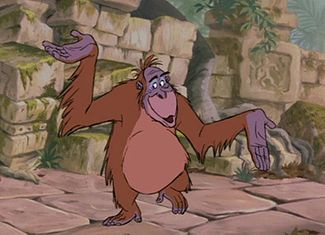
\includegraphics[scale=0.5]{KingLouie}

                {\small \it I wanna walk like you, talk like you...}
            \end{center}
        \end{frame}
    \section{Standard \textit{Estimators}}
        \begin{frame}{Estimators, Regression}
            This is not a new idea!

            \begin{center}
            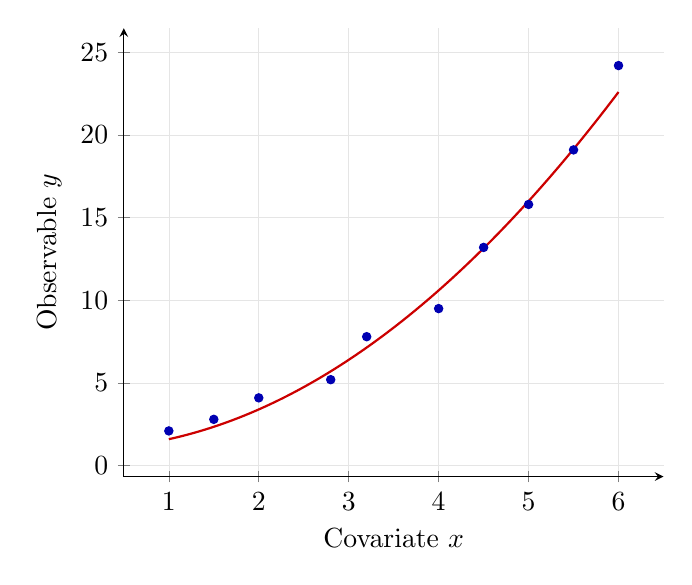
\begin{tikzpicture}
    \begin{axis}[
        xlabel={Covariate $x$},
        ylabel={Observable $y$},
        grid=both,
        grid style={line width=.1pt, draw=gray!10},
        major grid style={line width=.2pt, draw=gray!20},
        legend pos=north west,
        axis lines=left,
        enlarge x limits=0.1,
        enlarge y limits=0.1
    ]
        % The 'noisy' observed data
        \addplot[
            only marks,
            mark=*,
            mark size=1.5pt,
            blue!70!black
        ] coordinates {
            (1, 2.1) (1.5, 2.8) (2, 4.1) (2.8, 5.2) 
            (3.2, 7.8) (4, 9.5) (4.5, 13.2) (5, 15.8)
            (5.5, 19.1) (6, 24.2)
        };
        % \addlegendentry{Observed $\vec{T}$}

        % The 'fitted' regression curve
        % Using a simple y = 0.6x^2 + 1
        \addplot[
            red!80!black,
            thick,
            domain=1:6,
            samples=100
        ] {0.6*x^2 + 1};
        % \addlegendentry{Emulator $\hat{E}_M$}
        
    \end{axis}
\end{tikzpicture}
            \end{center}
        \end{frame}

        \begin{frame}{Machine Learning}
            In recent years\footnote{Though even this is becoming `old'}, we can use machine learning 
            \begin{itemize}
                \item Vast non-parametric models
                \pitem Condition it on observable data
                \begin{center}
                    
\includegraphics[scale=1.5]{LouieListens}
                    
                    {\small \it Now give me the secret, mancub 
                    
                    C'mon, clue me what to do}
                \end{center}
                \item Hope it learns the correct behaviour
            \end{itemize}
        \end{frame}

        \begin{frame}{The Limitation}

            \begin{block}{Distributions, not means}
                If $\hat{M}$ is stochastic, then $\vec{y}$ is not a number - it is a \textit{realisation on a random process}. 

                These methods serve only to predict the mean, $\mathbb{E}(\vec{y})$, not the distributions around that point.
            \end{block}

            \centering 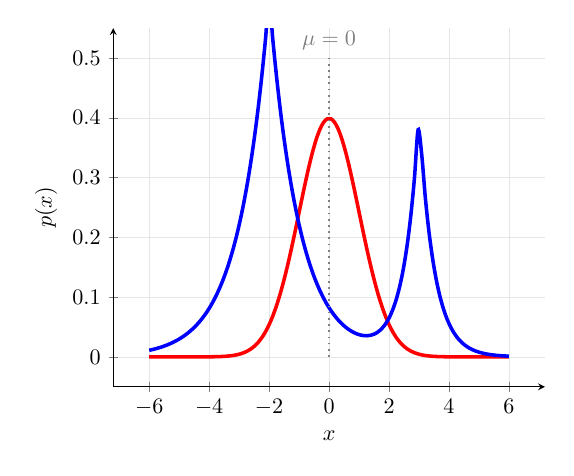
\begin{tikzpicture}[scale=0.8]
    \begin{axis}[
        xlabel={$x$},
        ylabel={$p(x)$},
        grid=both,
        grid style={line width=.1pt, draw=gray!10},
        major grid style={line width=.2pt, draw=gray!20},
        legend pos=north west,
        axis lines=left,
        enlarge x limits=0.1,
        enlarge y limits=0.1,
        xmin=-6, xmax=6, % Focus the plot range
        ymin=0, ymax=0.5, % Set vertical range
        ytick={0, 0.1, 0.2, 0.3, 0.4, 0.5} % Customize ticks for clarity
    ]
        
        % 1. Normal (Gaussian) Distribution: Mean=0, StdDev=1
        \addplot [
            domain=-6:6,
            samples=100,
            smooth,
            ultra thick,
            red,
        ] {1/(1*sqrt(2*pi)) * exp(-0.5*((x-0)/1)^2)};

        % 2. Laplace Distribution (Double Exponential): Mean=0, Scale=1
        % Equation: 1/(2*b) * exp(-|x-mu|/b)
        \addplot [
            domain=-6:6,
            samples=100,
            smooth,
            ultra thick,
            blue,
            % dashed
        ] {0.4 * exp(-abs(x-3)/0.5) + 0.6 * exp(-abs(x+2)/1)};
        
        % Vertical line indicating the shared mean
        \draw [gray, dotted, thick] (axis cs:0, 0) -- (axis cs:0, 0.5) node[anchor=south, gray] {$\mu=0$};

    \end{axis}
\end{tikzpicture}
        \end{frame}
        
        
    \section{Standard \textit{Predictors}}
        \begin{frame}{Machine Learning (Again)}
            There \textit{are} ML models which give distributions (Bayesian Neural Networks), but we may choose to avoid them:
            \begin{enumerate}
                \item Require lots of data (expensive - recall computing $\hat{M}$ is the bottleneck)
                \item Black boxes (aesthetically/scientifically dubious)
            \end{enumerate}
        \end{frame}
        \begin{frame}{Gaussian Processes}
            A modelling process where one assumes
            \begin{equation}
                \vec{y}(\vec{\pi}) \sim \mathcal{N}\left(\sum_i w_i(\pi) \vec{y}_i, \Sigma \right)
            \end{equation}
            % In short, compute an estimator of the mean, and then assume a Gaussian distribution at the end.

            Has many lovely properties, but fundamentally unsuitable for our work, as it assumes the distribution, rather than reconstructing it!


        \end{frame}

        \begin{frame}{Partition Models}
            Split the covariate space up into \textit{cells}
            \begin{center}
                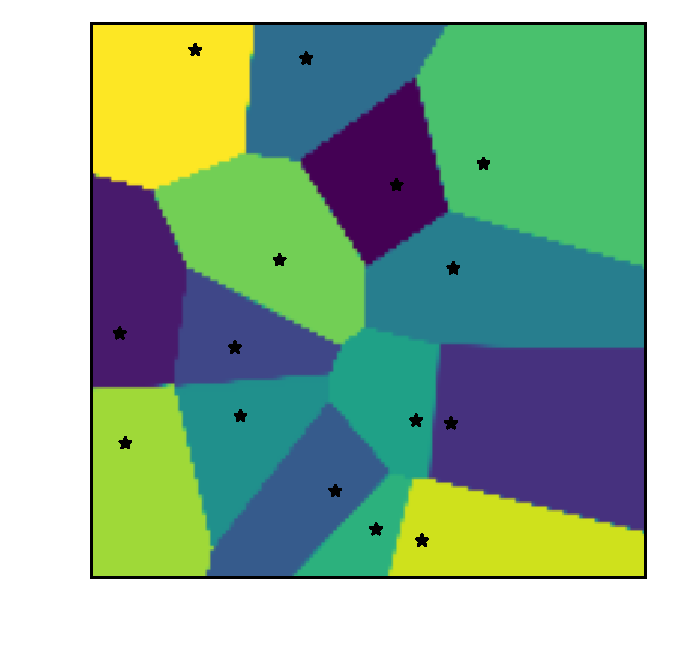
\includegraphics[scale=0.6]{tesselate}
            \end{center}
        \end{frame}
        \begin{frame}{Partition Models}
            Each cell fits their own PDF:
            \begin{center}
                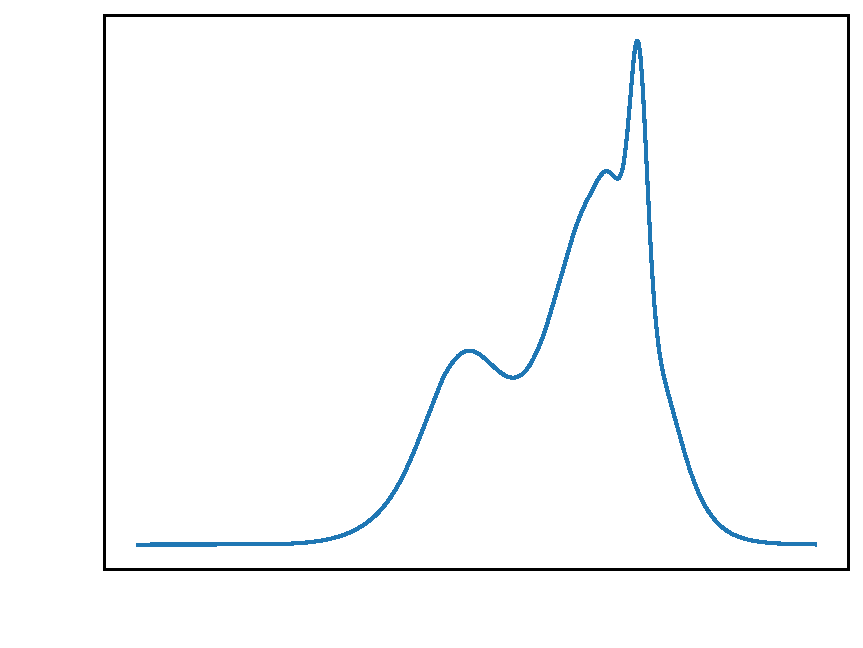
\includegraphics[scale=0.6]{query}
            \end{center}
        \end{frame}

        \begin{frame}{Mixture of Experts}
            Instead of a hard partition, MoE probabilistically assign the `problem' to an `expert':
            \begin{equation}
                p(y | \vec{x}) = \sum_i w_i(\vec{x}) p_i
            \end{equation}
            The $w_i$ give different weights to the `expert opinion' at different points in covariate space, coming to a different consensus. 

            Standard MoE uses Neural Networks to determine $w_i$ (via complex partitioning of a learned hyperplane projection)
        \end{frame}
    
    \section{Models into Emulators}
        \begin{frame}{Models are not Emulators}
            \begin{block}{Important!}
                The above models \textit{are not emulators}. They provide ways to model the best-fit posterior distribution, conditioned on the observed data:

                $$ \text{Model}_{\vec{\Theta}}(\vec{x}) = p(\vec{y} | \vec{x}, \vec{\Theta})$$
            \end{block}
            \begin{center}
                 \begin{center}
                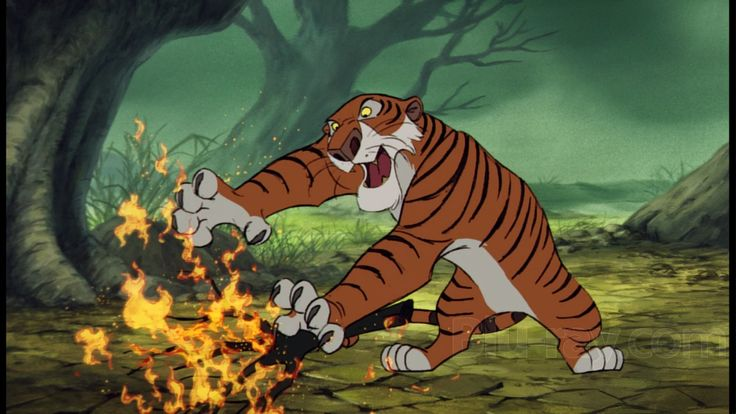
\includegraphics[scale=0.2]{sherekhan_fire.jpg}
            \end{center}

                \it \small What I desire is man's red fire

                To make my dream come true
            \end{center}
        \end{frame}
        \begin{frame}{The Secret of Man's Red Fire}
            What we need it the \textit{posterior predictive} distribution. The distribution conditioned \textit{only} on the data:
            \pause\begin{equation}
                \text{Emulator}(\vec{x}) = p(\vec{y} | \vec{x}) = \int\text{Model}_{\vec{\Theta}}(\vec{x}) \mathrm d \vec{\Theta}
            \end{equation}
            \pause \begin{center}
                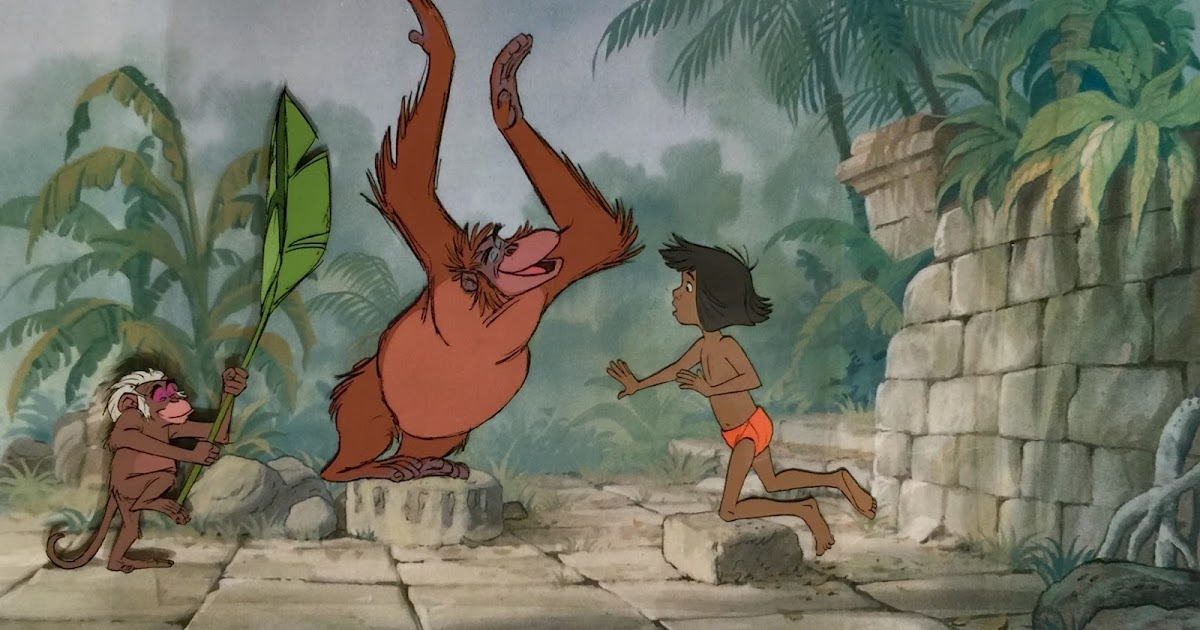
\includegraphics[scale=0.15]{happyLouie.jpg}

                \it \small An ape like me

                Can learn to be human too
            \end{center}
        \end{frame}

    \section{The FADE Emulator}
    \begin{frame}{Our Requirements}
        We needed an emulator which can:
        \begin{enumerate}
            \pitem Reconstruct probability distribution function 
            \pitem Allow both smooth and near-discontinuous changes in behaviour  
            \pitem Inherit `expert knowledge' to reduce training requirements
            \pitem Be interpretable and accessible
        \end{enumerate}
    \end{frame}

    \begin{frame}{Department of Experts}
        A middle ground between partitioning and MoE models. We allow each expert to belong to a `department' (a partition - which may have many experts within it), but also allow them to `spend time' between departments.

        The weight of an expert in the sum is then:
        \begin{equation}
            w_i(\vec{x}) = \sum_{\text{dep. } k} P(\vec{x} \in k) \times  \frac{P(i \in k) P(i \text{ knows } \vec{x})}{\sum_j P(j \in k) P(j \text{ knows } \vec{x})}
        \end{equation}
        These probabilities can be learned by the machine
    \end{frame}
    \begin{frame}{The Clever Bit}
        This reduces trivially down into a standard MoE, with model parameters $\vec{\Theta}$
        \begin{equation}
            p(\vec{x}|\vec{\Theta}) = \sum_w w_i(\vec{x} | \Theta) p_i(\vec{x} | \vec{\Theta})
        \end{equation}
        The clever bit is that we allow each department to have their own `grammar' that they use to talk to interpret the covariance space. The distance metric in each space is:
        \begin{equation}
            d_k(\vec{x}, \vec{y}) = \sqrt{(\vec{x} - \vec{y})\cdot G_k (\vec{x} - \vec{y})}
        \end{equation} 
        Where $G_k$ is a learned distance metric unique to each cell. 
    \end{frame}

    \begin{frame}{Why is this clever?}

        \begin{enumerate}
            \pitem Allows $w_i$ to encode highly nonlinear relationships in $\vec{x}$ \textit{without resorting to black-box machinery}. 
            \pitem The metrics are easily interpreted as covariance measures localised within a department. 
            \pitem Gives the same predictive power as a high dimensional hidden-layer neural network
            \pitem Constrained to produce `interpretable results'.
        \end{enumerate}
    \end{frame}

    \begin{frame}{A FADE Model}

        \begin{center}
            
            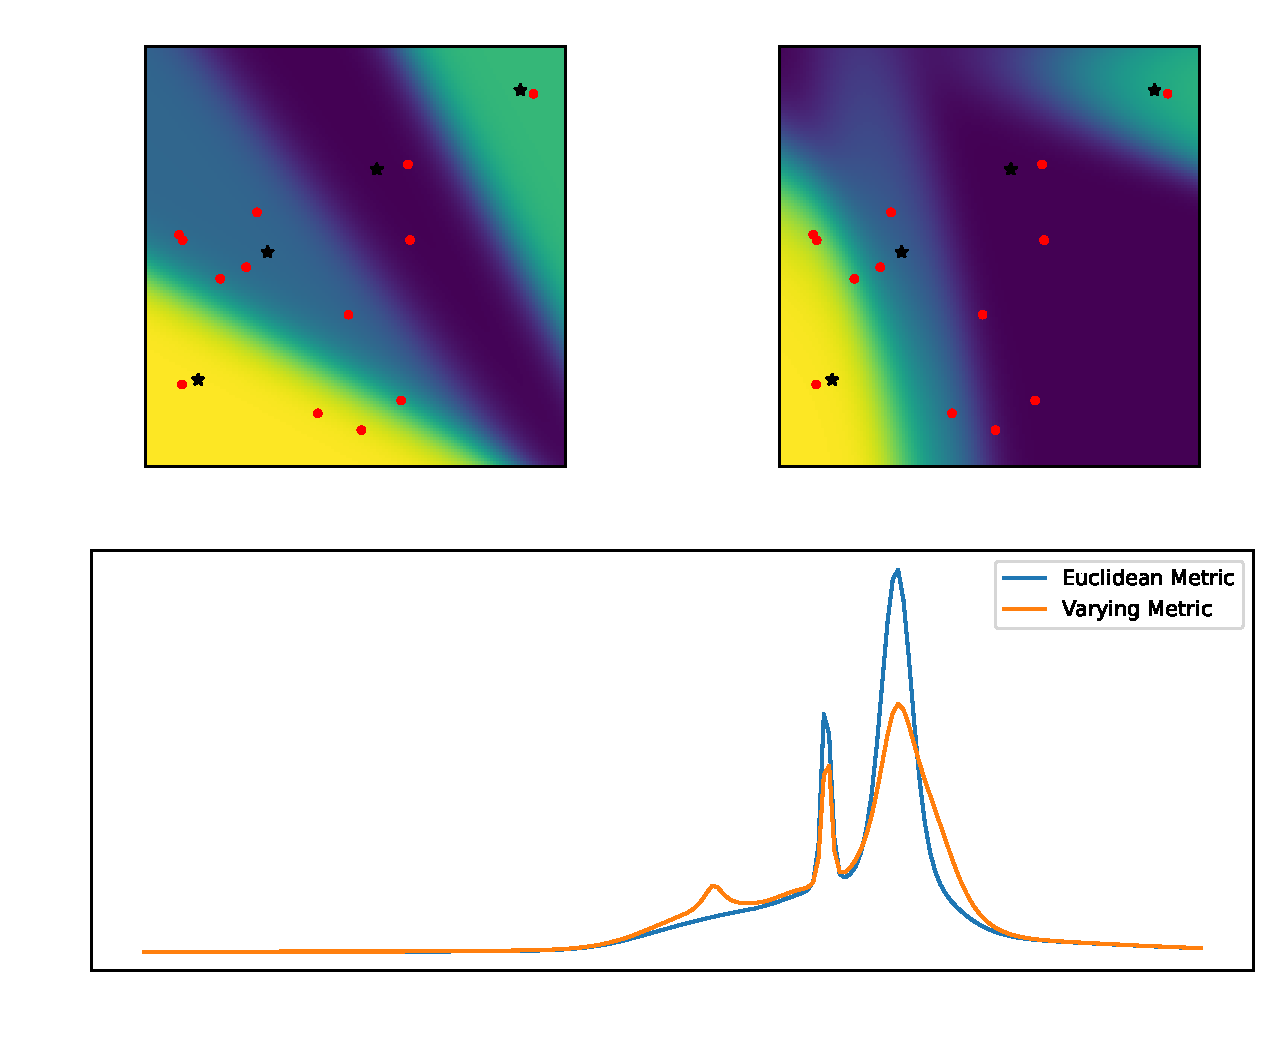
\includegraphics[scale=0.4]{metric_grids.pdf}
        \end{center}
    \end{frame}
\end{document}